\documentclass[english]{../thermomemo/thermomemo}
% \pdfminorversion=4
\usepackage[utf8]{inputenc}

\usepackage{amsmath}
%\input{mathdef}
\usepackage[per-mode=symbol]{siunitx}
\sisetup{per-mode=symbol}
\DeclareSIUnit{\ppm}{ppm}
\usepackage[numbers]{natbib}
\usepackage{amsmath}
\usepackage{amssymb}
\usepackage{array}% improves tabular environment.
\usepackage{dcolumn}% also improves tabular environment, with decimal centring.
\usepackage{chemformula}     % For easy typing of chemical formulae
\usepackage{booktabs}
\usepackage{a4wide}
\usepackage{xspace}
\usepackage{todonotes}
\presetkeys{todonotes}{inline}{}
\usepackage{subcaption,caption}
%\pdfminorversion=4
\usepackage{tikz}
\usetikzlibrary{arrows}
\usetikzlibrary{snakes}
\usepackage{verbatim}
\usepackage{hyperref}
\hypersetup{
  colorlinks=true,
  linkcolor=blue,
  urlcolor=blue,
  citecolor=blue
}
\usepackage{blkarray, bigstrut}
\usepackage{mhchem}
%
%\newcommand*{\od}[3][]{\frac{\mathrm{d}^{#1}#2}{\mathrm{d}{#3}^{#1}}}% ordinary derivative
\newcommand*{\od}[3][]{\frac{\dif^{#1}#2}{\dif{#3}^{#1}}}% ordinary derivative
\newcommand*{\pd}[3][]{\frac{\partial^{#1}#2}{\partial{#3}^{#1}}}% partial derivative
\newcommand*{\pdt}[3][]{{\partial^{#1}#2}/{\partial{#3}^{#1}}}% partial
                                % derivative for inline use.
\newcommand{\pone}[3]{\frac{\partial #1}{\partial #2}_{#3}}% partial
                                % derivative with information of
                                % constant variables
\newcommand{\ponel}[3]{\frac{\partial #1}{\partial #2}\bigg|_{#3}} % partial derivative with informatio of constant variable. A line is added.
\newcommand{\ptwo}[3]{\frac{\partial^{2} #1}{\partial #2 \partial
    #3}} % partial differential in two different variables
\newcommand{\pdn}[3]{\frac{\partial^{#1}#2}{\partial{#3}^{#1}}}% partial derivative

% Total derivative:
\newcommand*{\ttd}[2]{\frac{\mathrm{D} #1}{\mathrm{D} #2}}
\newcommand*{\td}[2]{\frac{\mathrm{d} #1}{\mathrm{d} #2}}
\newcommand*{\ddt}{\frac{\partial}{\partial t}}
\newcommand*{\ddx}{\frac{\partial}{\partial x}}
% Vectors etc:
% For Computer Modern:

\DeclareMathAlphabet{\mathsfsl}{OT1}{cmss}{m}{sl}
\renewcommand*{\vec}[1]{\boldsymbol{#1}}%
\newcommand*{\vektor}[1]{\boldsymbol{#1}}%
\newcommand*{\tensor}[1]{\mathsfsl{#1}}% 2. order tensor
\newcommand*{\matr}[1]{\tensor{#1}}% matrix
\renewcommand*{\div}{\boldsymbol{\nabla\cdot}}% divergence
\newcommand*{\grad}{\boldsymbol{\nabla}}% gradient
% fancy differential from Claudio Beccari, TUGboat:
% adjusts spacing automatically
\makeatletter
\newcommand*{\dif}{\@ifnextchar^{\DIfF}{\DIfF^{}}}
\def\DIfF^#1{\mathop{\mathrm{\mathstrut d}}\nolimits^{#1}\gobblesp@ce}
\def\gobblesp@ce{\futurelet\diffarg\opsp@ce}
\def\opsp@ce{%
  \let\DiffSpace\!%
  \ifx\diffarg(%
    \let\DiffSpace\relax
  \else
    \ifx\diffarg[%
      \let\DiffSpace\relax
    \else
      \ifx\diffarg\{%
        \let\DiffSpace\relax
      \fi\fi\fi\DiffSpace}
\makeatother
%
\newcommand*{\me}{\mathrm{e}}% e is not a variable (2.718281828...)
%\newcommand*{\mi}{\mathrm{i}}%  nor i (\sqrt{-1})
\newcommand*{\mpi}{\uppi}% nor pi (3.141592...) (works for for Lucida)
%
% lav tekst-indeks/subscript/pedex
\newcommand*{\ped}[1]{\ensuremath{_{\text{#1}}}}
% høy tekst-indeks/superscript/apex
\newcommand*{\ap}[1]{\ensuremath{^{\text{#1}}}}
\newcommand*{\apr}[1]{\ensuremath{^{\mathrm{#1}}}}
\newcommand*{\pedr}[1]{\ensuremath{_{\mathrm{#1}}}}
%
\newcommand*{\volfrac}{\alpha}% volume fraction
\newcommand*{\surften}{\sigma}% coeff. of surface tension
\newcommand*{\curv}{\kappa}% curvature
\newcommand*{\ls}{\phi}% level-set function
\newcommand*{\ep}{\Phi}% electric potential
\newcommand*{\perm}{\varepsilon}% electric permittivity
\newcommand*{\visc}{\mu}% molecular (dymamic) viscosity
\newcommand*{\kvisc}{\nu}% kinematic viscosity
\newcommand*{\cfl}{C}% CFL number

\newcommand*{\cons}{\vec U}
\newcommand*{\flux}{\vec F}
\newcommand*{\dens}{\rho}
\newcommand*{\svol}{\ensuremath v}
\newcommand*{\temp}{\ensuremath T}
\newcommand*{\vel}{\ensuremath u}
\newcommand*{\mom}{\dens\vel}
\newcommand*{\toten}{\ensuremath E}
\newcommand*{\inten}{\ensuremath e}
\newcommand*{\press}{\ensuremath p}
\renewcommand*{\ss}{\ensuremath a}
\newcommand*{\jac}{\matr A}
%
\newcommand*{\abs}[1]{\lvert#1\rvert}
\newcommand*{\bigabs}[1]{\bigl\lvert#1\bigr\rvert}
\newcommand*{\biggabs}[1]{\biggl\lvert#1\biggr\rvert}
\newcommand*{\norm}[1]{\lVert#1\rVert}
%
\newcommand*{\e}[1]{\times 10^{#1}}
\newcommand*{\ex}[1]{\times 10^{#1}}%shorthand -- for use e.g. in tables
\newcommand*{\exi}[1]{10^{#1}}%shorthand -- for use e.g. in tables
\newcommand*{\nondim}[1]{\ensuremath{\mathit{#1}}}% italic iflg. ISO. (???)
\newcommand*{\rey}{\nondim{Re}}
\newcommand*{\acro}[1]{\textsc{\MakeLowercase{#1}}}%acronyms etc.

\newcommand{\nto}{\ensuremath{\mbox{N}_{\mbox{\scriptsize 2}}}}
\newcommand{\chfire}{\ensuremath{\mbox{CH}_{\mbox{\scriptsize 4}}}}
%\newcommand*{\checked}{\ding{51}}
\newcommand{\celsius}{\ensuremath{^\circ\text{C}}}
%\newcommand{\clap}{Clapeyron~}
\newcommand{\subl}{\ensuremath{\text{sub}}}
\newcommand{\spec}{\text{spec}}
\newcommand{\sat}{\text{sat}}
\newcommand{\sol}{\text{sol}}
\newcommand{\liq}{\text{liq}}
\newcommand{\vap}{\text{vap}}
\newcommand{\amb}{\text{amb}}
\newcommand{\tr}{\text{tr}}
\newcommand{\crit}{\text{crit}}
\newcommand{\entr}{\ensuremath{\text{s}}}
\newcommand{\fus}{\text{fus}}
\newcommand{\flash}[1]{\ensuremath{#1\text{-flash}}}
\newcommand{\spce}[2]{\ensuremath{#1\, #2\text{ space}}}
\newcommand{\wrpt}{\text{with respec to~}}
\newcommand{\hyd}{\text{H}}
\newcommand{\wat}{\text{W}}
\newcommand{\mix}{\text{M}}
\newcommand{\ice}{\text{ice}}
\newcommand{\free}{{\ice/\liq}}

\title{Thermopack hydrate model}
\author{Morten Hammer}
\graphicspath{{gfx/}}

\begin{document}
\frontmatter

\section{Introduction}
The current memo introduces the Thermopack hydrate model, which
applies the van der Waals and Platteeuw method to determine the onset
of hydrate formation. The approach is similar to the model described
by \citet{Chapoy2012}. It is important to note that only \ce{CO2} is
considered as a guest molecule in the hydrate cages. Hydrates formed
with other guest molecules, such as \ce{CH4} or \ce{H2S}, are not
accounted for, even if these species are present in the mixture. This
limitation arises both from the absence of necessary parameterization
and the fact that the numerical methods are not configured to handle
hydrates formed with different guest molecules.

\section{Hydrate model}
The main equations of the hydrate model are given in this section.

The equilibrium condition of hydrate formation is equality between the
chemical potentials of water in the hydrate phase $\mu_\wat^\hyd$, and
water in the fluid mixture,
$\mu_\wat^\mix$,
\begin{equation}
\label{eq:hydform}
\mu_\wat^\hyd = \mu_\wat^\mix.
\end{equation}
Equation \eqref{eq:hydform} can be split into three separate
contributions, where each contribution represent a hypothetical
sub-process of the hydrate formation \citet{Sloan2008}:
\begin{equation}
\label{eq:hydsplit}
\mu_\wat^\hyd - \mu_\wat^\mix = \left( \mu_\wat^\free - \mu_\wat^\mix
\right) + \left( \mu_\wat^\beta - \mu_\wat^\free \right) + \left(
  \mu_\wat^\hyd - \mu_\wat^\beta \right) = 0.
\end{equation}

\begin{itemize}
\item \textbf{Term 1} $\left(\mu_\wat^\free - \mu_\wat^\mix\right)$: Formation of pure and free water (ice
  or liquid) from the VLLE mixture.
\item \textbf{Term 2} $\left(\mu_\wat^\beta - \mu_\wat^\free\right)$: Formation of an empty hydrate
  lattice from pure water.
\item \textbf{Term 3} $\left(\mu_\wat^\hyd - \mu_\wat^\beta\right)$: Formation of the
  hydrate-clathrate from the empty hydrate lattice.
\end{itemize}

It should be noted that since we are looking at the difference between
chemical potentials, all three terms can be modelled separately. The
three pairs must individually have the same reference state. Since
the reference states cancel, the pairs can have different reference
states.

If we choose to look at the fugacity directly, the equilibrium
condition becomes,
\begin{equation}
\label{eq:fug}
f_\wat^\mix = f_\wat^\hyd,
\end{equation}
with the hydrate fugacity
\begin{equation}
\label{eq:fug_hyd}
f_\wat^\hyd = f_\wat^\free e^{\left(\frac{\mu_\wat^\hyd - \mu_\wat^\beta}{RT}\right)} e^{\left(\frac{\mu_\wat^\beta - \mu_\wat^\free}{RT}\right)} .
\end{equation}

\subsection{Term 1 - Formation of free water}
The fugacity of free water can be modeled from
an suitable Equation of State (EoS) available in Thermopack.
\begin{equation}
  \label{eq:freewatform}
   f_\wat^\free = \text{min} \left( f_\wat^\liq, f_\wat^\ice \right)
\end{equation}
Here $R$ is the universal gas constant, and $T$ is the temperature,
$f$ is the fugacity.

To calculate the ice fugacity, the EoS by \citet{Feistel2006} have
been used, while the fluid fugacity can be calculated from multiple
EoSs.

\subsection{Poynting correction}
To account for ice, the Poynting correction given in the PhD-thesis by
\citet{Haghighi2009} can also be used. The Poynting correction uses the
\citet{Wagner1994} sublimation correlation to predict the fugacity
change of the assumed incompressible solid phase. It is important to
note that the predicted saturation pressure at 273.16\unit{\celsius}
for pure water, depends on the choice of EoS. It is
therefore necessary to calculate the saturation pressure at
273.16\unit{\celsius} from the EoS and apply this in the ice
model. Otherwise there will be a discontinuity in the fugacity over
the melting line.

\subsection{Term 2 - Formation of an empty hydrate
  lattice from pure water}
The change in chemical potential associated with the formation of an
empty hydrate lattice from pure water is modeled as follows:
\begin{equation}
  \label{eq:emptylattics}
  \frac{\mu_\wat^\beta - \mu_\wat^\free}{R T} = \frac{\Delta
    \mu_\wat^{\beta_0 - \ice_0/\liq_0}}{R T_0} -
  \overset{T}{\underset{T_0}{\int}} \frac{\Delta
    h_\wat^{\beta - \free}}{R T^2} dT + \overset{P}{\underset{P_0}{\int}} \frac{\Delta
    v_\wat^{\beta - \free}}{R T} dP.
\end{equation}
Here $h$ is the molar enthalpy, $v$ is the molar volume, and the
reference state $\left( T_0, P_0\right)$ is the triple point of
water. The enthalpy difference is modeled as,
\begin{equation}
  \label{eq:latticeformation}
    \Delta h_\wat^{\beta - \free} = \Delta h_\wat^{\beta_0 -
      \ice_0/\liq_0} + \overset{T}{\underset{T_0}{\int}} \Delta
    Cp_\wat^{\beta - \free} dT.
\end{equation}
The heat capacity difference, $\Delta Cp_\wat^{\beta - \free}$, is
modeled as linear function in temperature \cite{Holder1980}
\begin{equation}
  \label{eq:heatcap}
    \Delta Cp_\wat^{\beta - \free} = A_{Cp} + B_{Cp}\left( T - T_0\right).
\end{equation}
The parameters used for the integration is found in Table
\ref{tab:empty_lattice}. The triple point temperature is set to $T_0$
= \SI{273.16}{\kelvin}. The triple point pressure is calculated as the
saturation pressure at the triple temperature, and will be close to
the experimental value of $P_0$ = \SI{611.73}{\pascal}.
\begin{table}[tbp]
  \centering
  \caption{Reference properties for empty hydrate lattice from ice or
    water \cite{Haghighi2009} }
  \begin{tabular}{lll}
    \toprule
     & ice & water \\
    \midrule
    $\Delta \mu_\wat^{\beta_0 - \ice_0/\liq_0} (\unit{J/mol})$ & 1297
    & 1297 \\
    $\Delta h_\wat^{\beta_0 - \ice_0/\liq_0} (\unit{J/mol})$ & 1389 & -4620.5 \\
    $\Delta v_\wat^{\beta - \free} (\unit{cm^3/mol})$ & 3.0  &
  4.601\\
    $A_{Cp} (\unit{J/mol})$ & 0.565 & -37.32 \\
    $B_{Cp} (\unit{J/(mol K)})$ & 0.002 & 0.179\\
    \bottomrule
  \end{tabular}
  \label{tab:empty_lattice}
\end{table}

It should be noted that the discontinuous value of $\Delta v_\wat$ will
give a small discontinuity in the hydrate fugacity.

\subsection{Term 3 - Formation of the hydrate-clathrate from the empty
  hydrate lattice}
The change in chemical potential for the formation of the
hydrate-clathrate from the empty hydrate lattice is derived from
statistical thermodynamics:
\begin{equation}
  \label{eq:term3}
    \Delta \mu_\wat^{\beta - \hyd} = -RT \underset{i}{\sum}v_i \ln
    \left( 1- \underset{j}{\sum} \theta_{i,j} \right).
\end{equation}
The first sum is over small and lager cavities, and $v_i$ is here the number of
type $i$ cavities per water molecule, which is $1/23$ for small cavities
and $3/23$ for large cavities in structure I hydrates.
The fractional filling of cavity $i$ by component $j$ is given by an
Langmuir adsorption isotherm:
\begin{equation}
  \label{eq:theta}
    \theta_{i,j} = \frac{C_{i,j} f_j}{1 + \underset{k}{\sum} C_{i,k} f_k }
\end{equation}
The Kihara potential model is used to calculate the Langmuir
parameters $C_{i,j}$. See \citet{McKoy1963} and
\citet[Sec. 5.1.4]{Sloan2008}. Kihara potential parameters are taken from
multiple sources \citet{Sloan2008}, \citet{Avlonitis1994a},
\citet{Kalorazi1995}, \citet{Jager2013}.

\section{Isopleth hydrate appearance curve}
In order to map the hydrate appearance curve given an overall
composition, intersections with the fluid phase diagram are determined
and appearance curves are mapped from these intersections. Examples of
such plots are given in
\path{thermopack/addon/pyExamples/hydrate_curves.py}. See
Figures~\ref{fig:hydrate_co2} for a pure \ce{CO2} example and
Figure~\ref{fig:hydrate_co2_n2} for example of a binary mixture.

\begin{figure}[ht]
  \centering
  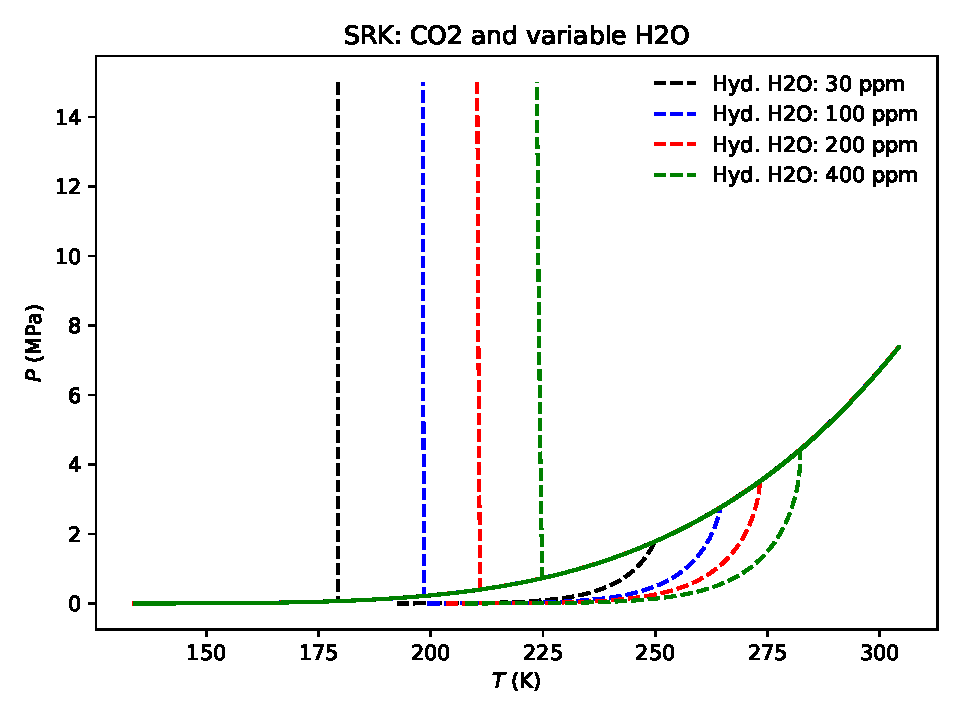
\includegraphics[width=0.6\textwidth]{hydrate_co2}
  \caption{Hydrate apperance curves in pure \ce{CO2}. Four hydrate
    curves are plotted for the water content
    \SIlist{30;100;200;400}{\ppm}}.
  \label{fig:hydrate_co2}
\end{figure}

\begin{figure}[ht]
  \centering
  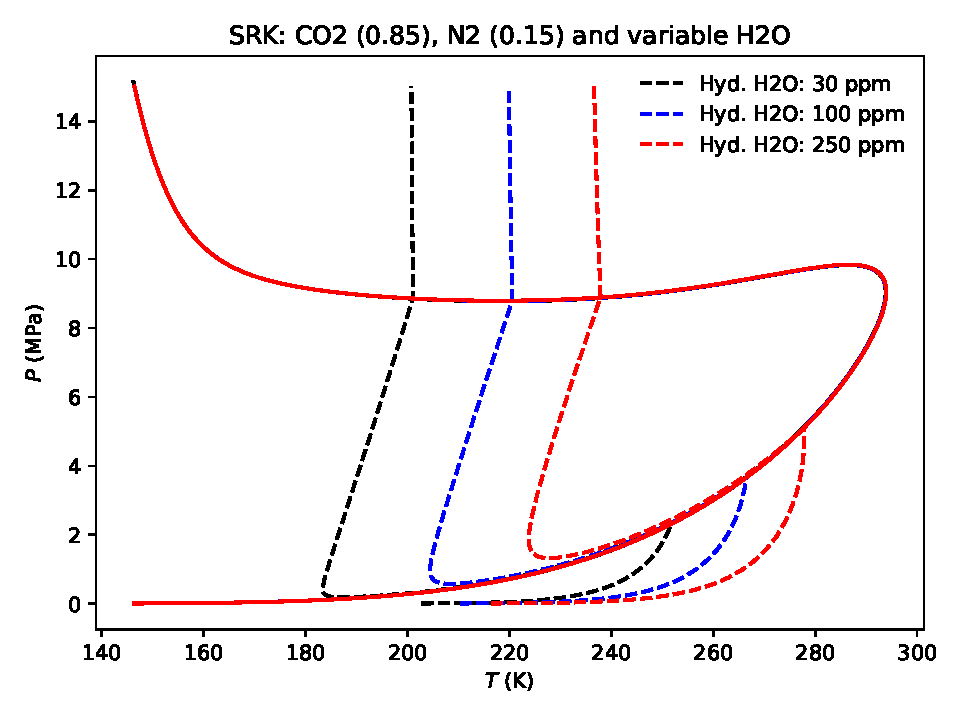
\includegraphics[width=0.6\textwidth]{hydrate_co2_n2}
  \caption{Illustration of hydrate apperance in a binary
    \ce{CO2}-\ce{N2} mixture. The mole fraction vector of the mixture
    is $\left[0.85,0.15\right]$. Three hydrate curves are plotted for
    the water content \SIlist{30;100;250}{\ppm}.}
  \label{fig:hydrate_co2_n2}
\end{figure}

\clearpage
\bibliographystyle{plainnat}
\bibliography{../thermopack}

\end{document}
